\documentclass[11pt,compress,t,notes=noshow, aspectratio=169, xcolor=table]{beamer}
\newcommand{\btVFill}{\vskip0pt plus 1filll}
\newcommand\hmmax{0}
\newcommand\bmmax{0}
\usepackage{../../style/lmu-lecture}
\usepackage{siunitx}
% Defines macros and environments
% This file is included in slides and exercises

% Rarely used fontstyle for R packages, used only in 
% - forests/slides-forests-benchmark.tex
% - exercises/single-exercises/methods_l_1.Rnw
% - slides/cart/attic/slides_extra_trees.Rnw
\newcommand{\pkg}[1]{{\fontseries{b}\selectfont #1}}

% Spacing helpers, used often (mostly in exercises for \dlz)
\newcommand{\lz}{\vspace{0.5cm}} % vertical space (used often in slides)
\newcommand{\dlz}{\vspace{1cm}}  % double vertical space (used often in exercises, never in slides)
\newcommand{\oneliner}[1] % Oneliner for important statements, used e.g. in iml, algods
{\begin{block}{}\begin{center}\begin{Large}#1\end{Large}\end{center}\end{block}}

% Don't know if this is used or needed, remove?
% textcolor that works in mathmode
% https://tex.stackexchange.com/a/261480
% Used e.g. in forests/slides-forests-bagging.tex
% [...] \textcolor{blue}{\tfrac{1}{M}\sum^M_{m} [...]
% \makeatletter
% \renewcommand*{\@textcolor}[3]{%
%   \protect\leavevmode
%   \begingroup
%     \color#1{#2}#3%
%   \endgroup
% }
% \makeatother


\title{Interpretable Machine Learning}
% \author{LMU}
%\institute{\href{https://compstat-lmu.github.io/lecture_iml/}{compstat-lmu.github.io/lecture\_iml}}
\date{}

\begin{document}

% TODO
\newcommand{\titlefigure}{figure_man/global_shap_depend_season.pdf}
% \newcommand{\learninggoals}{
% \item Get an intuition of additive feature attributions
% \item Understand the concept of Kernel SHAP
% \item Ability to interpret SHAP plots
% \item Global SHAP methods
% }
\newcommand{\learninggoals}{
\item Understand how SHAP values can be aggregated for global model interpretation
\item Learn global SHAP visualizations: feature importance, summary, and dependence plots
\item Recognize advantages and limitations of global SHAP explanations
}

\lecturechapter{Global SHAP}
\lecture{Interpretable Machine Learning}

\begin{frame}{Global SHAP \citebutton{Lundberg et al. 2018}{https://doi.org/10.48550/arXiv.1802.03888}}
\textbf{Idea: }
\begin{itemize}
    \item Run SHAP for every observation and thereby get a matrix of Shapley values
    \item The matrix has one row per data observation and one column per feature
    \item We can interpret the model globally by analyzing the Shapley value matrix
\end{itemize}
\vspace{2cm}
$$
\Phi =
\begin{bmatrix}
    \phi_{11} & \phi_{12} & \phi_{13} & \dots  & \phi_{1p} \\
    \phi_{21} & \phi_{22} & \phi_{23} & \dots  & \phi_{2p} \\
    \vdots & \vdots & \vdots & \ddots & \vdots \\
    \phi_{n1} & \phi_{n2} & \phi_{n3} & \dots  & \phi_{np} \\
\end{bmatrix}
$$

 \end{frame}

 \begin{frame}{Feature Importance}

\begin{onlyenv}<1>
\textbf{Idea:} Average the absolute Shapley values of each feature over all observations. This corresponds to calculating averages column by column in matrix $\Phi$
$$
I_{j}=\frac{1}{n} \sum_{i=1}^{n}\left|\phi_{j}^{(i)}\right|
$$
\end{onlyenv}

\begin{onlyenv}<2>
\textbf{Interpretation:}
\begin{itemize}
    \item Features \enquote{temp} and \enquote{year} have highest influence on the model's prediction
    \item Shapley FI does not provide information on direction of the effect\\
    $\leadsto$ Provides a feature ranking based on the magnitude of the Shapley values %similar to PFI
    \item Shapley FI is based only on model predictions\\
    Note: Other FI measures are based on model's performance (loss)
\end{itemize}
 
\end{onlyenv}


\btVFill

\begin{figure}
    \centering
    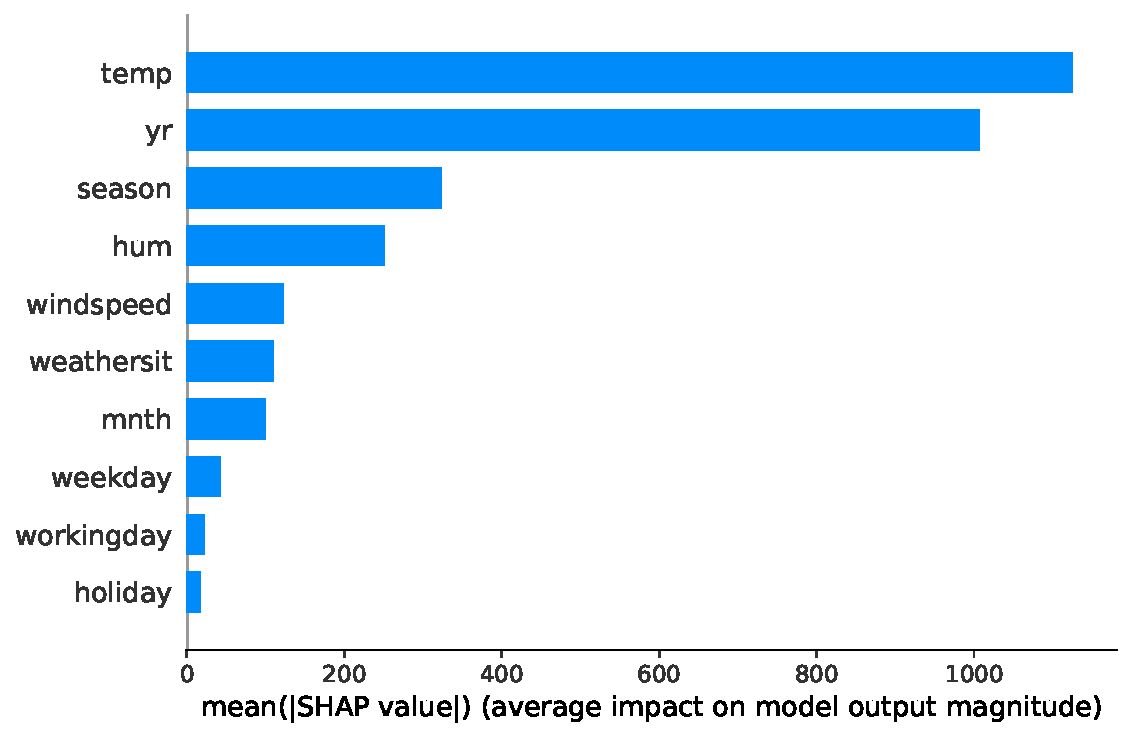
\includegraphics[width=0.5\columnwidth]{figure_man/global_shap_fi.pdf}
\end{figure}

\end{frame}
 
\begin{frame}{Summary Plot}
\begin{onlyenv}<1>
Combines feature importance with feature effects
\begin{itemize}
    \item Each point is a Shapley value for a feature and an observation
    \item The color represents the value of the feature from low to high
    \item Overlapping points are jittered in y-axis direction
\end{itemize}
\end{onlyenv}

\begin{onlyenv}<2>
\textbf{Interpretation:}\\
\begin{itemize}
    \item Low temp have a negative impact; high temp lead to more bike rentals
    \item Year: two point clouds for 2011 (low value) and 2012 (high value)\\
    \item Categorical features are gray (no low/high value)
    \item High humidity has a huge negative impact on bike rentals
    \item Low humidity has a rather minor positive impact on bike rentals
\end{itemize}
 
\end{onlyenv}

\btVFill

\begin{figure}
    \centering
    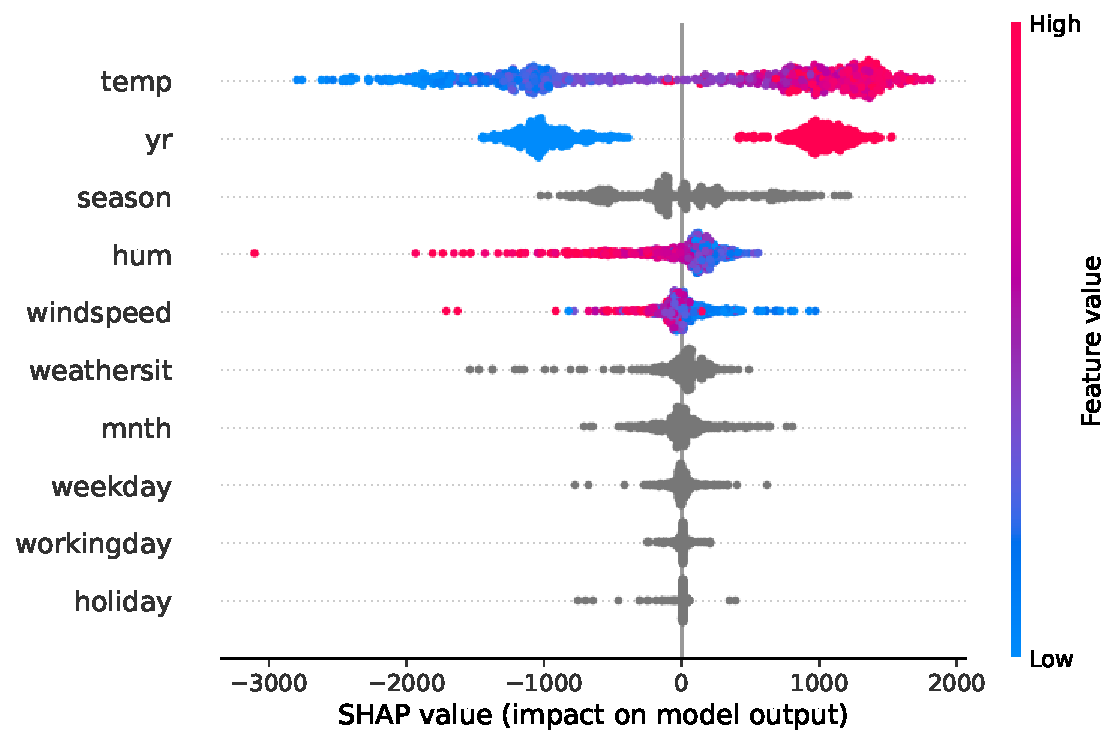
\includegraphics[width=0.5\columnwidth]{figure_man/global_shap_jitter.pdf}
    
\end{figure}
\end{frame} 

% \begin{frame}{Dependence Plot}

% \begin{onlyenv}<1>
% \begin{itemize}
%     \item Visualize the marginal contribution of a feature similar to the PDP 
%     \item Plot a point with the feature value on the x-axis and the corresponding Shapley value on the y-axis
% \end{itemize}

% \end{onlyenv}

% \begin{onlyenv}<2>
% \textbf{Interpretation:}\\
% \begin{itemize}
%     \item Increasing temperatures induce increasing bike rentals until $25^\circ\text{C}$
%     \item If it gets too hot, the bike rentals decrease
% \end{itemize}
% \end{onlyenv}

% % \begin{onlyenv}<3>
% % \textbf{Interpretation:}\\
% % \begin{itemize}
% %     \item We can colour the observations by a second feature to detect interactions
% %     \item Visibly the temperatures interaction with the season is very strong
% %     \item In summer, when temperatures rise, we see an increase in the model's SHAP values, indicating more bike rentals. By contrast, winter's lower temperatures translate into negative SHAP contributions, suggesting fewer rentals.
% % \end{itemize}
% % \end{onlyenv}


% \btVFill
% \begin{onlyenv}<1-2>
% \begin{figure}
%     \centering
%     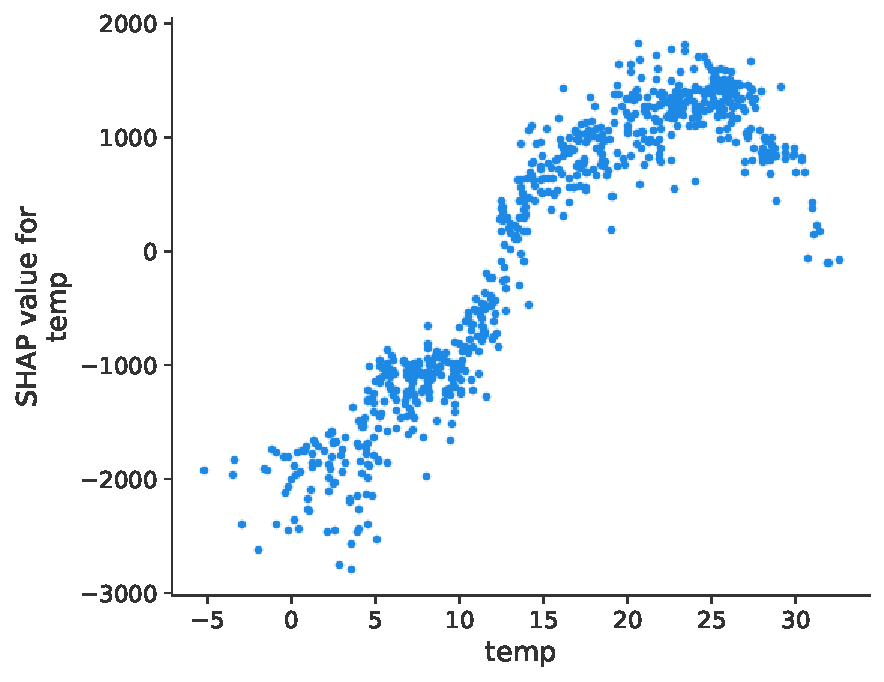
\includegraphics[width=0.5\columnwidth]{figure_man/global_shap_depend.pdf}
% \end{figure}
% \end{onlyenv}

% % \begin{onlyenv}<3>
% % \begin{figure}
% %     \centering
% %     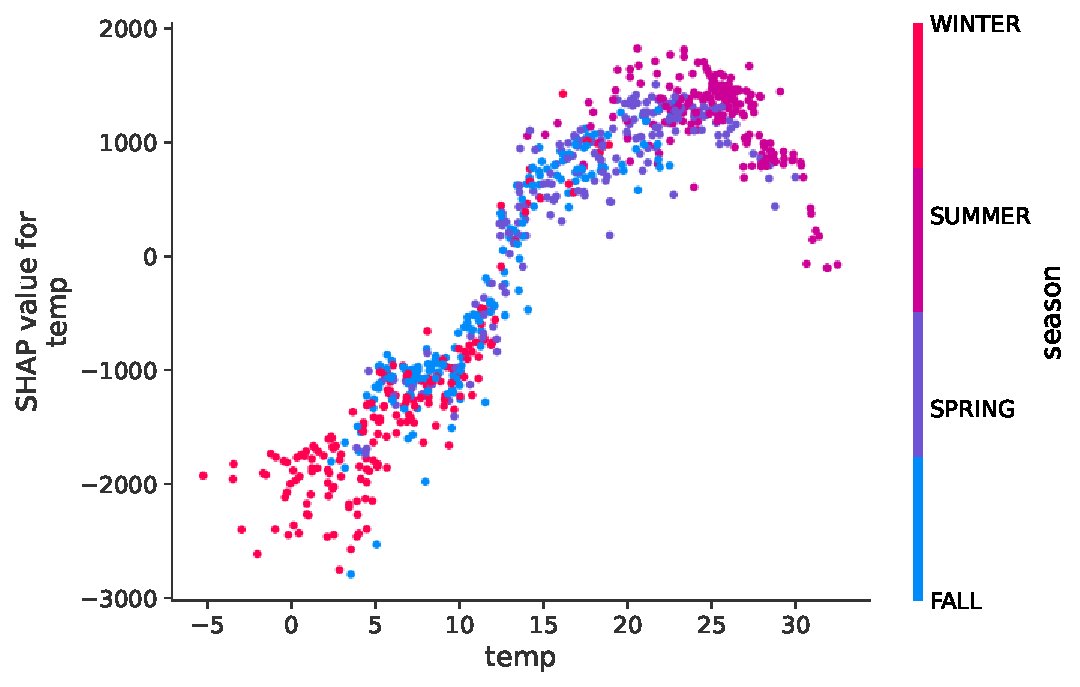
\includegraphics[width=0.5\columnwidth]{figure_man/global_shap_depend_season.pdf}
% % \end{figure}
% % \end{onlyenv}
% \end{frame}


\begin{frame}{Dependence Plot: Effect + Interaction}

\textbf{Interpretation of SHAP Dependence Plot (Feature = Temperature)}

\begin{itemize}
  \item<1-> Plot points with feature value on x-axis and corresponding SHAP value on y-axis
  %\textbf{X-axis:} feature value (temp); \textbf{Y-axis:} SHAP value for temp
  %\item<1-> Each point = one observation
  \item<2-> Shows how temp influences bike rentals $\leadsto$ Marginal effect similar to PD plot
  \item<2-> SHAP values increase with temp until $\approx$25°C: higher temp $\leadsto$ higher predictions
  \item<2-> After $\approx$25°C, SHAP values decrease slightly %$\leadsto$ decreasing effect
  \item<3-> Interaction with \textbf{season} is visible (via color-encoded observations):
    \begin{itemize}
        \item In \textcolor{violet}{summer}, higher temperatures decrease bike rentals
        \item In \textcolor{blue}{winter}, higher temperatures increase bike rentals
    \end{itemize}
\end{itemize}

\btVFill
\begin{figure}
    \centering
     \includegraphics<1-2>[width=0.4\textwidth]{figure_man/global_shap_depend.pdf}
    \includegraphics<3->[width=0.5\textwidth]{figure_man/global_shap_depend_season.pdf}
\end{figure}

\end{frame}



\begin{frame}{Discussion}

\textbf{Advantages}

\begin{itemize}
    \item Retains local accuracy: SHAP values exactly decompose predictions
    \item Aggregating local SHAP values yields global model insights\\
    $\leadsto$ Visual diagnostics: feature importance, summary plot, dependence plots
    \item Efficient for tree-based models via TreeSHAP\\
    (See \citebutton{Lundberg et al 2018}{https://doi.org/10.48550/arXiv.1802.03888} and for intuitive explanation \citebutton{Sukumar: TreeSHAP}{https://medium.com/analytics-vidhya/shap-part-3-tree-shap-3af9bcd7cd9b})
    \item Unifies feature attribution under a consistent additive framework
    
    %\item All the advantages of Shapley values
    %\item Unify the field of interpretable machine learning in the class of additive feature attribution methods
    %\item Has a fast implementation for tree-based models
    %\item Various global interpretation methods
    \item Can be used for images \citebutton{SHAP image examples}{https://github.com/shap/shap/tree/master/notebooks/image_examples}  and text \citebutton{SHAP text examples}{https://github.com/shap/shap/tree/master/notebooks/text_examples}
\end{itemize}

\medskip

\textbf{Disadvantages}

\begin{itemize}
  \item KernelSHAP is inefficient for large datasets or complex models
   \item Ignores feature dependencies in marginal sampling (interventional SHAP)
   \item Conditional sampling (observational SHAP) is difficult in practice (would require estimating a conditional distribution)
 
   %\item Disadvantages of Shapley values also apply to SHAP
    % \begin{itemize}
    %     \item Shapley values can be misinterpreted and access to data is needed to compute them for new data (not if TreeSHAP is used)
    % \end{itemize}
    %\item KernelSHAP is slow (TreeSHAP can be used as a faster alternative for tree-based models  -- and for an intuitive explanation  \citebutton{see Sukumar: TreeSHAP}{https://medium.com/analytics-vidhya/shap-part-3-tree-shap-3af9bcd7cd9b})
    %\item KernelSHAP ignores feature dependence 
    %\item TreeSHAP can produce unintuitive feature attributions
    %\item It is possible to create intentionally misleading interpretations with SHAP, which can hide biases \citebutton{Slack et al. 2020}{https://doi.org/10.1145/3375627.3375830}
\end{itemize}


\end{frame}

\endlecture
\end{document}
